\subsection{Prognosekarten \& Cell Difference Maps}
\begin{figure}[H]
    \centering
    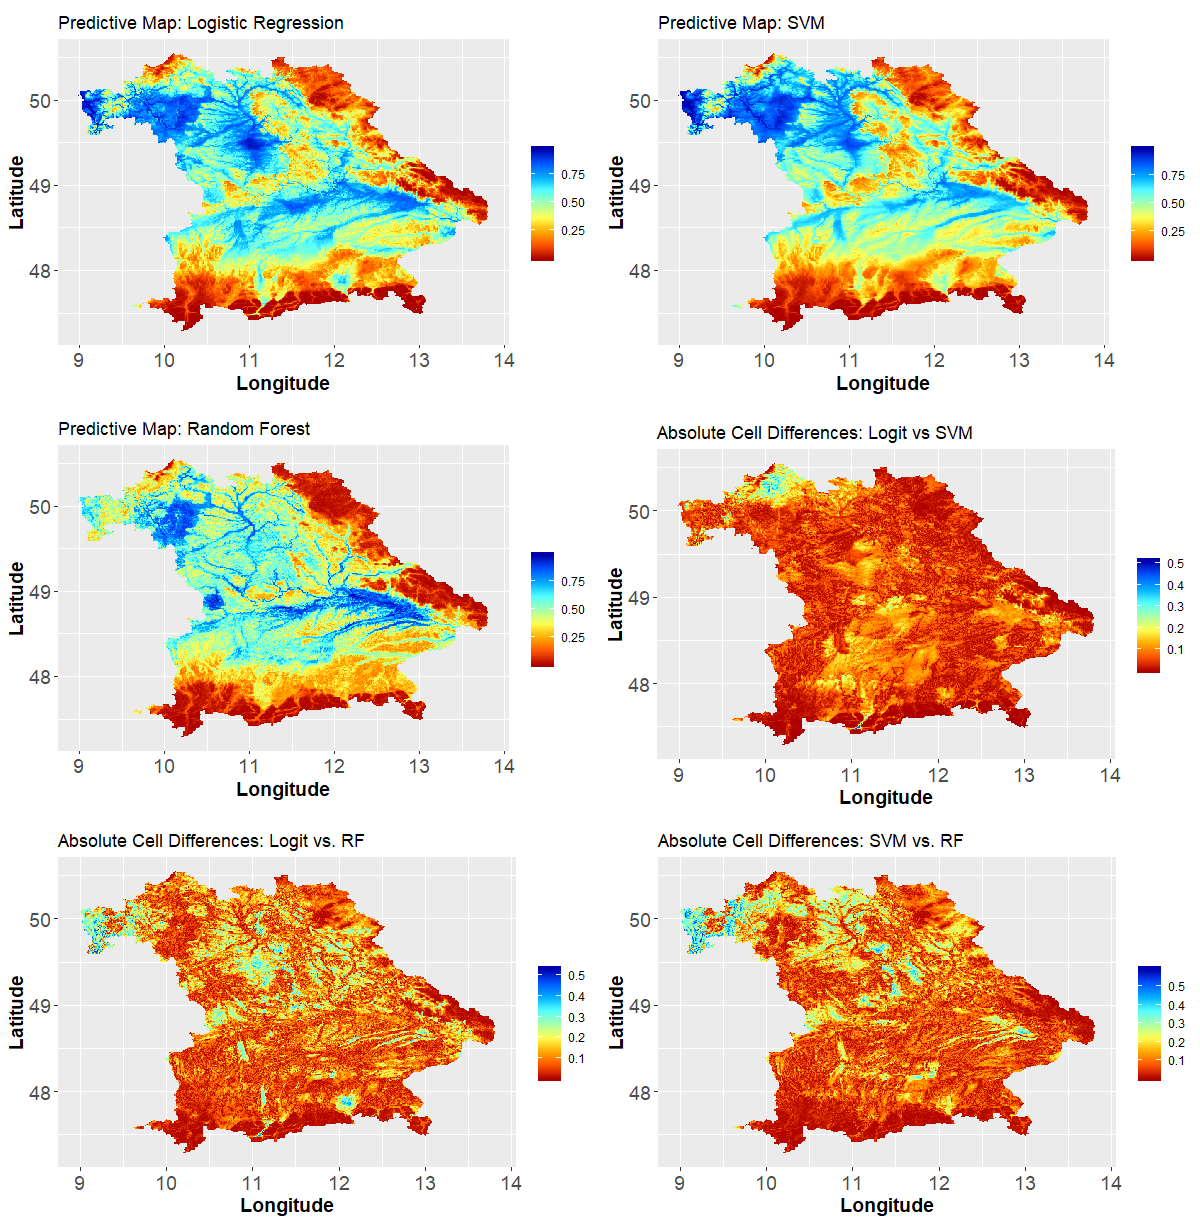
\includegraphics[width = 15cm, height = 19cm]{Figures/pmapsfinal.png}
    \caption{Die Prognosen der Modelle für den gesamten Rasterdatensatz. In den Karten oben links sind die geschätzten Wahrscheinlichkeiten für die Zugehörigkeiten der Rasterzellen zur Klasse ``Sites''. Die drei Karten in der unteren rechten Ecke visualisieren die absoluten Differenzen der Schätzergebnisse von Modell zu Modell.}
    \label{pmapsfinal}
\end{figure}
Eine praktische Eigenschaft von Rasterdaten ist die ``Vollständigkeit'' für das interessierende Areal. Im Normalfall müsste interpoliert werden um lückenlose Prognosen aufstellen zu können, da der Datensatz komplett aus Rasterlayern konstruiert wurde konnten so Vorhersagekarten für ganz Bayern generiert werden. Die Farbe der Karten kodiert die Wahrscheinlichkeit der Zugehörigkeit der einzelnen Pixel zur Klasse ``Site''. Rot lässt geschätzte Wahrscheinlichkeiten nahe 0 vermuten, Blau dagegen nahe 1. Sowohl das logistische Modell, als auch der Support Vector Classifier schätzten Prognoseareale mit ``weicheren'' Grenzen die eher gedämpft ineinander übergehen. Der Random Forest Classifier schätzte dagegen eine kontrastreichere Prognosekarte mit klarer erkennbaren Grenzen. Dies bestätigten auch die Cell Difference Maps. In diesen Karten wurden die absoluten Rasterzelldifferenzen der Prognosen paarweise aufgetragen. Logistisches Modell und Support Vector Classifier produzierten für weite Teile Bayerns sehr ähnliche Ergebnisse -- die mittleren Zelldifferenzen betrugen nur 0.06. Dies steht im Kontrast zu den Vorhersagen des Random Forest Classifiers. Hier lassen sich an den deutlich kontrastreicheren Cell Difference Maps sogar einige Gewässer identifizieren. \\
Die in Abbildung \ref{pmapsfinal} sichtbaren Karten zu SV- und RF Classifier wurden jeweils aus Modellen mit durch repeated spatial Cross Validation erhaltenen Hyperparametern erstellt. Es schien wenig sinnvoll auch predictive Maps für standard CV mit in die Analyse aufzunehmen da aus diesen, wie im nächsten Abschnitt diskutiert wird, zu hohe Werte für die Prognosegüte hervorgehen. 

\subsection{Modellperformance}

Sowohl für Hyperparametertuning, als auch für den allgemeinen Vergleich der predictive Performance der Modelle wurden, mit den in Abschnitt 3.4 erklärten Crossvalidation Verfahren, die ``Area under the Curve'' (AUC) Werte der ROC Kurve errechnet. Die 5-fold CV wurde für jedes der Modelle und Resamplingverfahren 100 mal wiederholt. Die Verteilungen der erhaltenen Schätzwerte sind in \ref{performanceviz} abgebildet.

\begin{figure}[H]
    \centering
    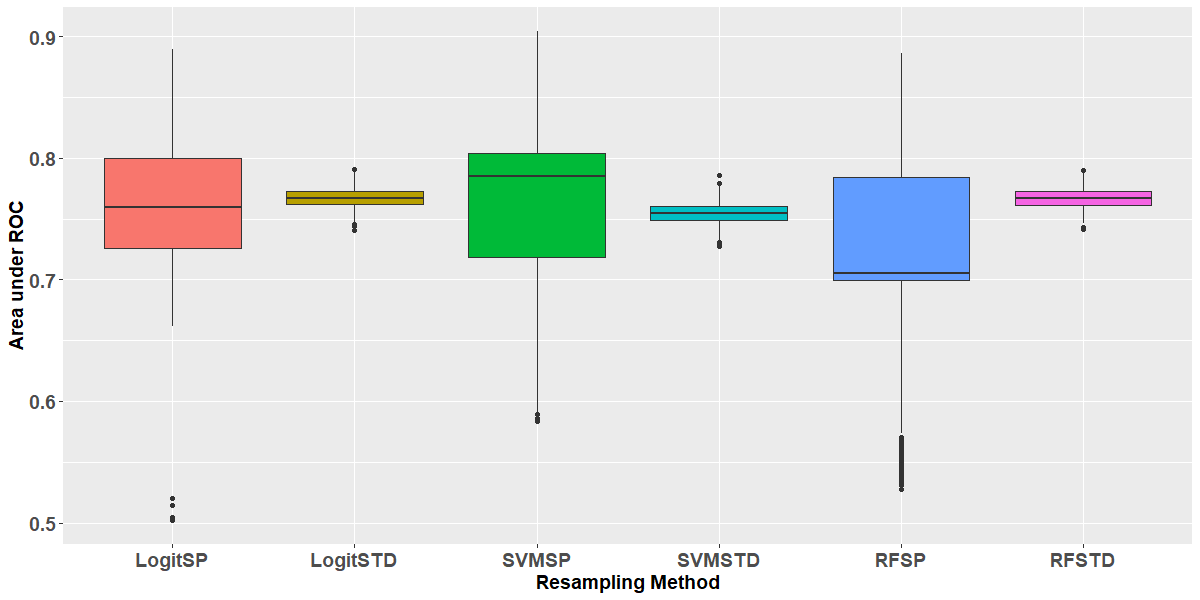
\includegraphics[width = 15cm, height = 7.5cm]{Figures/resamplingcomparison.png}
    \caption{Predictive Performance Vergleich der Modelle. ``SP'' entspricht repeated spatial CV; ``STD'' entspricht repeated standard CV}
    \label{performanceviz}
\end{figure}

Wie erwartet bewirkte die räumlich zusammenhängende CV eine Korrektur der mittleren Prognoseperformance der Modelle für logistisches- und Random Forest Modell nach unten. Überraschend ist der mittlere Performancegain für den SVM Klassifikator. Zur Erklärung dieses Phänomens wären weitere Untersuchungen nötig. Die Variation aller spatial Schätzer steigerte sich drastisch verglichen mit den Schätzern aus den standard CV Verfahren. Dies könnte ein Indiz dafür sein, dass ein sehr großes Forschungsareal wie Gesamtbayern nicht optimal für diese Resamplingmethode ist. Eventuell könnte es sinnvoll sein, das Forschungsareal vorab in kleinere Areale zu unterteilen (Ähnlich der nested CV) und dann innerhalb dieser kleineren Areale zu modellieren. Auch an Abbildung \ref{resamplingviz} wird erkennbar, dass sich bei repeated spatial CV Trainingsdatensätze ergeben können in denen ein Großteil der Sites, enthalten ist. Die allgemeine räumliche Verteilung der Sites scheint in Kombination mit dem gewählten Areal eventuell problematisch für dieses Verfahren zu sein. 